\documentclass[aspectratio=169, 14pt]{beamer} % 16:9 aspect ratio to match modern screens
\usefonttheme{serif}

% --- Packages ---
\usepackage{pifont}
\usepackage[T1]{fontenc}
\usepackage[utf8]{inputenc}

\usepackage{lmodern}

\usepackage{dsfont}
\usepackage{xcolor}
\usepackage{tcolorbox}
\tcbuselibrary{skins, theorems}
\usepackage{multimedia} % Included for video support
\usepackage{fontawesome5}
\usepackage[normalem]{ulem} % The normalem option keeps your \emph{} styling normal
\usepackage{cancel}
\usepackage{amsmath}
\usepackage{mathtools}
\usepackage{circuitikz}
\usepackage{pgfplots}
\pgfplotsset{compat=1.18}
\usepackage{pgfplotstable}
\usetikzlibrary{arrows.meta}
\usepackage{tkz-tab}
\usepackage{tikz}
\usepackage{tikz-cd}
\tikzstyle{lien}
=[->,>=stealth,rounded
corners=5pt,thick]
\tikzset{
	invisible/.style={opacity=0, text opacity=0},
	visible on/.style={alt={#1{}{invisible}}},
	alt/.code args={<#1>#2#3}{%
		\alt<#1>{\pgfkeysalso{#2}}{\pgfkeysalso{#3}}%
	},
}
\usepackage{amssymb}
\usetikzlibrary{arrows.meta, positioning, calc}
\usepackage{esvect}
\usepackage{graphicx}

\DeclareMathAlphabet{\mathpzc}{OT1}{pzc}{m}{it}

% --- Bibliography ---
\usepackage[
	backend=bibtex,
	giveninits=true,
	style=numeric,
	maxbibnames=99,
	mincitenames=1,
	maxcitenames=4
]{biblatex}
\addbibresource{bibi.bib}
\setbeamerfont{footnote}{size=\tiny}
\setbeamercolor{footnote mark}{fg=brandAccent}

% --- Color Definitions (from theme.scss) ---
\definecolor{brandAccent}{HTML}{D77E62}
\definecolor{brandPurple}{HTML}{7201A8}
\definecolor{brandAccentDark}{HTML}{B7654B}
% Approximating the transparent #e6a08a4a background
\colorlet{brandAccentLight}{brandAccent!5!white}
\colorlet{brandRed}{brandAccent!20!red}


\definecolor{Grad1}{HTML}{FFD200}
\definecolor{Grad2}{HTML}{F4A539}
\definecolor{Grad3}{HTML}{D37867}
\definecolor{Grad4}{HTML}{983494}
\definecolor{Grad5}{HTML}{7201A8}

% --- Beamer Color & Font Settings ---
\setbeamercolor{title}{fg=brandAccent}
\setbeamercolor{frametitle}{fg=brandAccent}
\setbeamercolor{structure}{fg=brandAccent} % Colors bullets and standard structural elements
\setbeamercolor{author}{fg=black}
\setbeamercolor{date}{fg=black}

% --- Link & Reference Styling ---
\renewcommand{\eqref}[1]{\hyperref[#1]{\color{brandAccent}(\ref*{#1})}}
\hypersetup{
	colorlinks=false,
	linkcolor=brandAccent,
	urlcolor=brandAccent,
	citecolor=brandAccent
}

% Clean up the presentation (removes navigation symbols)
\setbeamertemplate{navigation symbols}{}
\setbeamertemplate{footline}[page number]

% --- Custom Theorem Block (Replicating the CSS Bubble Style) ---
\newtcbtheorem{mythm}{Theorem}{
	enhanced,
	colback=brandAccentLight,
	colframe=brandAccent,
	boxrule=1pt,
	arc=4mm,          % 14px border radius
	auto outer arc,
	coltitle=white,
	colbacktitle=brandAccent,
	fonttitle=\bfseries\small,
	top=5mm,  % <--- INCREASES VERTICAL SPACE BETWEEN BUBBLE AND TEXT
	bottom=2mm, % Optional: gives a little breathing room at the bottom too
	% Pill-shaped floating title
	separator sign={},
	title style={borderline={0pt}{0pt}{brandAccent}, rounded corners, arc=2mm},
	attach boxed title to top left={xshift=4mm, yshift=-3mm},
	boxed title style={
		size=small,
		top=-0.5mm,    % <--- Shrink top padding
		bottom=-0.5mm, % <--- Shrink bottom padding
		left=1mm,     % <--- Shrink left padding
		right=1mm     % <--- Shrink right padding
	}
}{thm}
\newtcbtheorem{myprop}{Proposition}{
	enhanced,
	colback=brandAccentLight,
	colframe=brandAccent,
	boxrule=1pt,
	arc=4mm,          % 14px border radius
	auto outer arc,
	coltitle=white,
	colbacktitle=brandAccent,
	fonttitle=\bfseries\small,
	top=3mm,
	bottom=2mm,
	separator sign={},
	% Pill-shaped floating title
	title style={borderline={0pt}{0pt}{brandAccent}, rounded corners, arc=2mm},
	attach boxed title to top left={xshift=4mm, yshift=-3mm},
	boxed title style={
		size=small,
		top=-0.5mm,    % <--- Shrink top padding
		bottom=-0.5mm, % <--- Shrink bottom padding
		left=1mm,     % <--- Shrink left padding
		right=1mm     % <--- Shrink right padding
	}
}{prop}
\newtcbtheorem{myex}{Exemple}{
	enhanced,
	colback=brandAccentLight,
	colframe=brandAccent,
	boxrule=1pt,
	arc=4mm,          % 14px border radius
	auto outer arc,
	coltitle=white,
	colbacktitle=brandAccent,
	fonttitle=\bfseries\small,
	top=3mm,
	bottom=2mm,
	separator sign={},
	% Pill-shaped floating title
	title style={borderline={0pt}{0pt}{brandAccent}, rounded corners, arc=2mm},
	attach boxed title to top left={xshift=4mm, yshift=-3mm},
	boxed title style={
		size=small,
		top=-0.5mm,    % <--- Shrink top padding
		bottom=-0.5mm, % <--- Shrink bottom padding
		left=1mm,     % <--- Shrink left padding
		right=1mm     % <--- Shrink right padding
	}
}{ex}

% --- Maths ---
\def\argmin#1{{\underset{#1}{\mathrm{arg}\,\mathrm{min}\ }}}
\def\argmax#1{{\underset{#1}{\mathrm{arg}\,\mathrm{max}\ }}}
\def\d{\mathrm{d}}
\newcommand{\cev}[1]{\reflectbox{$\vec{\reflectbox{$#1$}}$}}
\newcommand{\rust}[1]{\textcolor{brandAccent}{#1}}
\newcommand{\purp}[1]{\textcolor{brandPurple}{#1}}
\renewcommand{\exp}[1]{\mathrm{exp}\left(#1\right)}
\renewcommand{\ln}[1]{\mathrm{ln}\left(#1\right)}
\newcommand{\myatop}[2]{
	\fontdimen10\textfont2=\fontdimen9\textfont2
	{\begingroup#1\endgroup\atop#2}}

% --- Title Information ---
\title{
	Des définitions, du vocabulaire et des exemples
}
\subtitle{Café des Sciences}
\author{Quentin Giton}
\institute{}
\date{6 Juin 2026}

\setbeamertemplate{page number in head/foot}{\insertframenumber{} / \inserttotalframenumber}
\setbeamertemplate{section in toc}{%
	\rust{\ding{43}}~\textcolor{black}{\inserttocsection}\par
}
\setbeamertemplate{subsection in toc}{%
	\hspace{1.2em}\rust{\ding{229}}~\textcolor{black}{\inserttocsubsection}\par
}

\begin{document}
	\begin{frame}
		\titlepage
	\end{frame}
	
	\begin{frame}{Plan}
		\tableofcontents
	\end{frame}

	\section{Algorithmes}
	
	
	\begin{frame}[t]{Algorithmes}
		\begin{columns}[T]
			\only<1->{
				\begin{column}{0.48\textwidth}
					\begin{myex*}{1}
						\begin{itemize}
							\item Choisir trois nombres $x_1,x_2,x_3$
							\item Multiplier :
							\begin{itemize}
								\item $x_1$ par $2$
								\item $x_2$ par $1$
								\item $x_3$ par $5$
							\end{itemize}
							\item Ajouter le tout
							\item Retrancher $10$
						\end{itemize}
					\end{myex*}
				\end{column}
			}
			\visible<2->{
				\begin{column}{0.48\textwidth}
					\begin{myex*}{2}
						\begin{itemize}
							\item Choisir un nombre $x$
							\item \textbf{Si} $x$ est pair :
							\begin{itemize}
								\item Diviser $x$ par $2$
							\end{itemize}
							\item \textbf{Sinon :}
							\begin{itemize}
								\item Multiplier $x$ par $2$
								\item Ajouter $1$
							\end{itemize}
							\item Répéter $5$ fois
						\end{itemize}
					\end{myex*}
				\end{column}
			}
		\end{columns}
	\end{frame}
	
	
	\section{Apprentissage Machine (ML)}
	\subsection{La régression linéaire}
	
	
	\begin{frame}[t]{La régression linéaire}
		\begin{columns}[T]
			\begin{column}{0.48\textwidth}
				\begin{center}
					\begin{figure}
						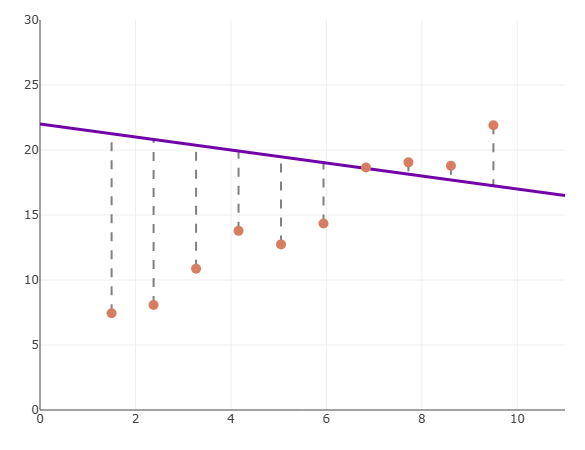
\includegraphics[scale=0.3]{images/Reg1.png}
					\end{figure}
					\only<3>{\textbf{MSE = 57,19}}
				\end{center}
			\end{column}
			\begin{column}{0.48\textwidth}
				\begin{center}
					\begin{figure}
						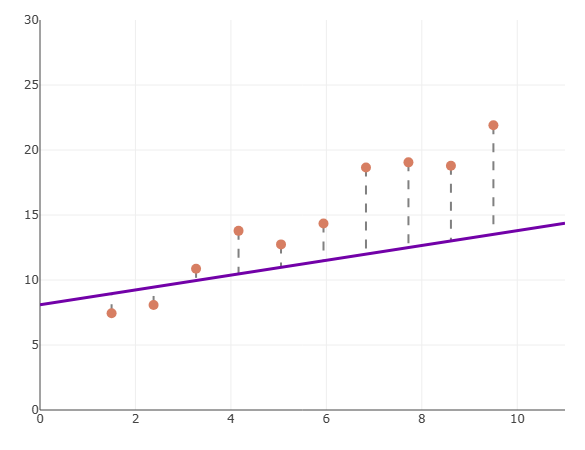
\includegraphics[scale=0.3]{images/Reg2.png}
					\end{figure}
					\only<3>{\textbf{MSE = 19,19}}
				\end{center}
			\end{column}
		\end{columns}
		\only<2>{
		\begin{equation*}
			\mathrm{MSE} = \min_{a,b} \sum_{i=1}^N \big( y_i - (ax_i+b) \big)^2
		\end{equation*}
		}
		\vspace{\baselineskip}
		\begin{center}
			\only<4>{\small\url{https://quentingiton.github.io/scripts/linear-regression}}
		\end{center}
	\end{frame}
	
	
	\subsection{L'importance du nombre de données}
	
	
	\begin{frame}[fragile]{L'importance du nombre de données}
		\begin{center}
			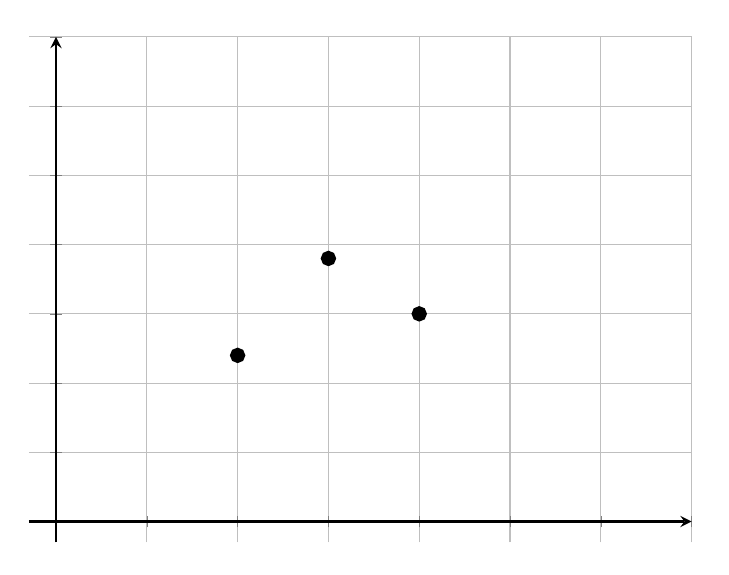
\begin{tikzpicture}[scale=1]
				\begin{axis}[
					axis lines = center,
					every axis plot/.append style={line width=1.5pt},
					xticklabels = \empty,
					yticklabels = \empty,
					xmin = -0.15, xmax = 3.5,
					ymin = -0.15, ymax = 3.5,
					domain = -0.15:3.5,
					samples = 100,
					grid = major,
					width = 10cm,
					height = 8cm,
					thick
					]
					
					\addplot [only marks] table {
						1 1.2
						1.5 1.9
						2 1.5
					};
					
				\end{axis}
			\end{tikzpicture}
		\end{center}
	\end{frame}
	
	
	\subsection{L'importance du nombre de paramètres}
	
	
	\begin{frame}{L'importance du nombre de paramètres}
		\begin{itemize}
			\item Plus il y a de paramètres, plus l'on peut décrire des formes complexes
		\end{itemize}
		\begin{center}
			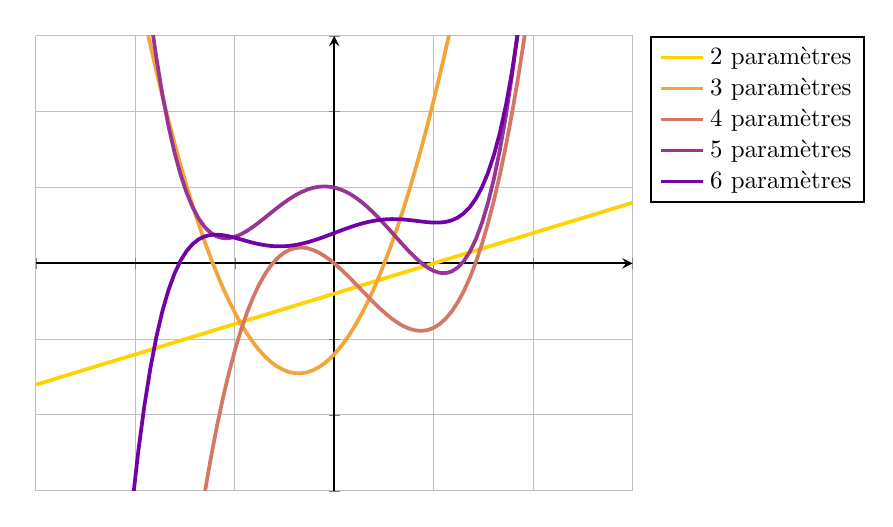
\begin{tikzpicture}[scale=0.9]
				\begin{axis}[
					axis lines = center,
					every axis plot/.append style={line width=1.5pt},
					xticklabels = \empty,
					yticklabels = \empty,
					xmin = -1.5, xmax = 1.5,
					ymin = -1.5, ymax = 1.5,
					domain = -1.5:1.5,
					samples = 100, % Augmenter pour lisser les courbes de haut degré
					legend pos = outer north east, % Place la légende à l'extérieur pour ne pas cacher les courbes
					legend cell align = {left},
					grid = major,
					width = 10cm,
					height = 8cm,
					thick
					]
					
					% Degré 1 (ax + b) -> 2 paramètres
					\addplot[color=Grad1] {0.4*x-0.2};
					\addlegendentry{2 paramètres}
					
					% Degré 2 (ax^2 + bx + c) -> 3 paramètres
					\addplot[color=Grad2] {3.9*x^2+1.4*x-0.6};
					\addlegendentry{3 paramètres}
					
					% Degré 3 -> 4 paramètres
					\addplot[color=Grad3] {5*x^3-2*x^2-1.1*x};
					\addlegendentry{4 paramètres}
					
					% Degré 4 -> 5 paramètres
					\addplot[color=Grad4] {5*x^4+0.3*x^3-3*x^2-0.3*x+0.5};
					\addlegendentry{5 paramètres}
					
					% Degré 5 -> 6 paramètres
					\addplot[color=Grad5] {4*x^5+0.3*x^4-2.6*x^3+0.5*x+0.2};
					\addlegendentry{6 paramètres}
					
				\end{axis}
			\end{tikzpicture}
		\end{center}
	\end{frame}
	
	
	\section{Réseaux de neurones}
	\subsection{Choix de la fonction de perte}
	\section{Modèles Génératifs}
	\section{Grands Modèles de Langage (LLM)}
	\section{Pour résumer}
	
	
	
\end{document}